% igs2eannalsguide.tex
% v4.00 3-sept-2015

\NeedsTeXFormat{LaTeX2e}

% check that the math fits the two-column format:
% \documentclass[annals,twocolumn]{igs}

% but use this version when submitting your article:
  \documentclass[annals,review,oneside]{igs}

% other options are available
%   authors printing on US letter size are advised 
%   to use the slightly shorter [letterpaper] option
% SINGLE COLUMN
%   \documentclass[annals]{igs}              
% SINGLE COLUMN, FEWER LINES/PAGE
%   \documentclass[annals,letterpaper]{igs} 
% DOUBLE COLUMN, FEWER LINES/PAGE
%   \documentclass[annals,twocolumn,letterpaper]{igs} 

  \usepackage{igsnatbib}
 \usepackage{amsmath}
% 
% check if we are compiling under latex or pdflatex
  \ifx\pdftexversion\undefined
    \usepackage[dvips]{graphicx}
  \else
    \usepackage[pdftex]{graphicx}
    \usepackage{epstopdf}
    \epstopdfsetup{suffix=}
  \fi

\usepackage{tikz}
% the default is for unnumbered section heads
% if you really must have numbered sections, remove
% the % from the beginning of the following command
% and insert the level of sections you wish to be
% numbered (up to 4):

% \setcounter{secnumdepth}{2}

\begin{document}

\title[Deglaciation of Helm]{Helm Glacier projected to vanish within a decade}

\author[gsc]{Jeffrey W. CROMPTON$^1$, Brian MENOUNOS$^{1,3,4}$, Mark EDNIE$^{2}$}

\affiliation{%
$^1$Geological Survey of Canada, Natural Resources Canada, Vancouver, British Columbia, Canada \\
$^2$Geological Survey of Canada, Natural Resources Canada, Ottawa, ON, Canada, \\
$^3$Department of Geography, Earth, and Environmental Science, University of Northern British Columbia, Prince George, British Columbia, Canada \\
$^4$ Hakai Institute, Campbell River, British Columbia, Canada \\
}


\abstract{Goodbye Helm, thanks for all the ice}

\maketitle

\section{Introduction}

Over the last four years, glaciers in Western Canada and the conterminous US lost twice as much mass as during the period 2010-2019  \citep{Menounos2025}. This mass loss occurred primarily through widespread surface thinning driven by warm, dry conditions and general darkening of glacier surfaces. In terms of surface area, Canada contains about 185,000 km$^{2}$ of glacierized terrain, about one quarter of the global total \citep{rgi70}.  Given the importance of glacier runoff to Canada's economy, the federal government established a network of glacier monitoring sites during the International Hydrological Decade (IHD) \citep{Ommanney1986}. These sites became operational in 1965 and, ten years later, the Government of Canada added Helm Glacier to its list of monitoring sites given its maritime environment (\cite{Ommanney2002}). Helm Glacier is a World Glacier Monitoring Service (WGMS) reference glacier and only one of four alpine glaciers in Canada to have monitoring record which exceeds 40 years.  In addition to their importance of recording  seasonal-to-annual response of glaciers to climate change, emph{In situ} glacier monitoring records provides seaonal-to-annual observations required for regional upscaling of glacier mass change \citep{Zemp2019}. The objectives of this short note is to describe recent changes of Helm Glacier and estimate when Helm Glacier is projected to disappear. 

\begin{figure}[H!]
\centering
\includegraphics[width=150mm,trim=0.1cm 0.1cm 0.1cm 0.1cm, clip=true]
{study_area_map.jpg}
\caption{\textbf{Inset map:} Helm Glacier (red star) within Garibaldi Provincial Park. \textbf{Background image:} PlaceScope color composite (NIR-R-G) of Helm Glacier [28 August, 2017] and surrounding terrain. Black solid and yellow dashed lines respectively denote glacier extent in 2024 and 1928 survey photo-topographc survey of the glacier \citep{Koch2009}. \textbf{Upper right images:} Oblique image (left) of Helm Glacier in 1910s (unknown photographer) and glacier extent from Google Earth Engine (6 Aug, 2019 imagery). 1910s image courtesy of City of Vancouver Archives}
\label{study_area_map}
\end{figure}

\section{Study area and Methods}

Helm Glacier (49$^{\circ}$57’29” N, 122$^{\circ}$59’13” W) lies on the western edge of Garibaldi Provincial Park in the Pacific Ranges of the southern Coast Mountains in the traditional territory of the Squamish Nation (Figure \ref{study_area_map}). The small (0.4 km$^{2}$) glacier's currently ranges in elevation from 1780\,m a.s.l. to 2150\,m a.s.l. 

\subsection{Glacier mapping mass balance surveys}

We digitized the extent of Helm Glacier from spaceborne (Landsat 5,7,8,9) and airborne ortho-imagery, the latter acquired by the Hakai-UNBC Airborne Coastal Observatory \citep{Donahue2023}. We take the product of the ground sampling distance of the imagery and the glaciers perimeter to reflect the uncertainty in our mapping. As described above, Helm Glacier represents a WGMS reference glacier where mass balance measurements follow the stratigraphic method \citep{Kaser2003}. The glacier's seasonal balances are derived from 6-8 ablation stakes positioned along the centreline of the glacier, snow depth probing and end-of-winter snow pits where snow density and stratigraphic observations are made. Those data are used to generate seasonal and annual mass balance for the glacier and by updating the glacier area every few years. 

\subsection{Ice-penetrating radar}

We completed an ice-penetrating radar survey of Helm Glacier on 21 May, 2025. The Blue Systems Integration Ltd. radar system uses resistively-loaded dipole antennas with a centre frequency of ~10 MHz, has 12-bit resolution and yields a sampling rate of up to 250 Megasamples per second. The radar system contains a single frequency GNSS system with an accuracy of $\pm$5 m. To increase the vertical accuracy for the glacier surface ($\pm$ 0.5\,m), we acquired airborne Lidar for the surface elevation of the glacier on 24 April, 2025. Details about methods used for Lidar acquisition can be found elsewhere \citep{Menounos2025}.  Observations of surface elevation change from a sonic depth ranger equipped with satellite telemetry \cite{Bevington2025a}, reveals about 1\,m of thinning between our Lidar and radar surveys. We processed the radar data with IceRadarAnalyzer 6.3.1, with an antenna spacing of 15\,m and assuming a velocity through ice at 1.68x10$^{8}$ m s$^{-1}$ \citep{Reynolds2011}. To increase the signal-to-noise ratio of the data, we averaged 128 stacks for each trace in the radargram and then applied gain and filtering for identification of bed reflectors. We completed crossover analysis (i.e. where two radar transects overlap) and propagated in quadrature  the uncertainty using one-quarter of the radar wavelength \cite{Reynolds2011} and uncertainty that arises from surface slope to yield an error of ice thickness of $\pm$ 4.5\,m.  2D linear interpolation of the ice thickness data yielded a map of ice thickness (10 m ground sampling distance - gsd ).  

\subsection{Projection of glacier disappearance}

To estimate when Helm Glacier is expected to vanish, we forward model the yearly surface elevation change of Helm Glacier using two approaches described below. Both of these approaches use surface elevation data obtained from repeat Lidar surveys of Helm Glacier completed at the end of ablation season in 2020--2024. These five autumn surveys provide elevation change maps for 2021, 2022, 2023 and 2024.  Those airborne surveys followed the same methods as those used for the 24 April, 2025 survey. As described below, elevation change at a given point can be equated to annual surface mass balance given the thinness of the glacier (i.e. negligible dynamics) and minimal extent of retained snow on the glacier (i.e. density-to-mass conversion is simplified). The elevation change maps are downsampled to 10 m gsd to match the ice thickness grid. Co-registration of elevation change maps used methods described in \cite{Nuth2011} and \cite{Hugonnet2022} available in the XDEM package (https://pypi.org/project/xdem/).

Our first approach averages the surface elevation change at each grid cell over the four year period, then simply differences this average elevation change from the ice thickness grid each year (method 1). Ice vanishes at a given grid cell when the total melt exceeds the ice thickness of the column. The error in area is simply taken recomputing the elevation change within the ice thickness error bounds of 4.5\,m. 

For the second approach, we use a regression model to predict elevation change $\mathbf{dh}^{y}$ based on the design matrix of observations $\mathbf{X}^{y}$ for each of the years $j=\{2021,\,2022,\,2023,\,2024\}$ for each of the $n$ grid cells (method 2). Linear regression can be used to model mass change at the regional \citep{Lliboutry1974,Anilkumar2023,Reynaud1986} to individual ablation stake scale \citep{Zekollari2018}. The matrix $\mathbf{X}^{y}$ is composed of slope ($\boldsymbol{\theta}^{y}$), orientation ($\boldsymbol{\alpha}^{y}$), positive-degree days ($\mathbf{PDD}^{y}$), shortwave radiation at the surface ($\mathbf{SW_{\downarrow}}^{y}$) and snow depth ($\mathbf{h}^{y}$). The regression $\mathbf{dh} = \mathbf{X} \boldsymbol{\beta} + \boldsymbol{\varepsilon}$ is computed on the matrix $\mathbf{X}$ and observations $\mathbf{dh}$ that are concatenated across the four-year record. The optimal coefficients are estimated through least-squares regression as, $\hat{\boldsymbol{\beta}} = (\mathbf{X}^\top \mathbf{X})^{-1} \mathbf{X}^\top \mathbf{M}$. The model is validated by modelling the surface change for each year individually as $\hat{\mathbf{M}}^{j} = \mathbf{X}^{j} \hat{\boldsymbol{\beta}}$, with the $R^2$ computed between the yearly difference in observed and modelled elevation change at each grid cell. 

PDDs are computed are summed in the time intervals given by the LiDAR acquisition dates as $\mathbf{PDD}^y = \frac{1}{24}\sum T(z)$ for $T>0^{\circ}$C. The temperature ($T$) is taken from dynamically downscaled hourly ERA-5 land temperatures \citep{Hersbach2020} given at the nearest grid point and lapsed up from 1550\,m to the elevation of each grid cell. Similar to the melt-season lapse rate computed by \cite{Shea2009} of -6.0$\mathrm{^{\circ}C\,km^{-1}}$, we calculate April to October lapse rates from a series of nearby weather stations as -5.8$\mathrm{^{\circ}C\,km^{-1}}$. Snow depth is estimated from yearly snow depth observations collected every April at six glacier centreline stake locations. A yearly snow depth field is computed as a function of elevation by linearly interpolating observations to grid cell elevations. The summer incoming shortwave radiation is computed my multiplying a shading factor matrix computed in the HORAYZON v1.2 model \citep{Steger2022} with the mean of the daily averaged downwelling shortwave radiation obtained from the nearest gridpoint of ERA5-Land reanalysis. Although the shading model and surface normal shortwave radiation both depend on surface slope and aspect, we include slope and aspect as individual columns in the design matrix to capture other mass balance processes like snow redistribution.

To forward model the ice loss, we start with the 2024 DEM and force the model with the average of the PDD fields from 2014 to 2024, all computed at the 2024 grid cell elevations from April 01 to October 31. The forcing for $\mathbf{SW_{\downarrow}}$ and the snow depth field $\mathbf{h}$ field are generated from averaging the 2020--2024 fields used in the regression model. At each step forward in time, we recompute the surface elevation, slope, aspect, $\mathbf{PDD}$ field and snow-depth field, but keep $\mathbf{SW_{\downarrow}}$ fixed in time. We estimate uncertainty in elevation change by initializing the ice thickness at the $\pm 4.5$\,m error bounds and by varying the lapse rate by $\pm 5\%$. 

\subsection{Mass balance sensitivity}
We test the net mass balance ($b_n$) sensitivity of our model to changes in temperature as $\mathrm{C_T} = \partial b_n/ \partial T$ and precipitation as $\mathrm{C_P} = \partial b_n/ \partial P$. Sensitivities are computed by varying the mean summer temperature and the mean winter accumulation of the model \citep[e.g.][]{Cuffey2010}. Numerical derivatives for $\mathrm{C_T}$ and $\mathrm{C_P}$ are computed for the current temperature and accumulation conditions. We test the sensitivity of i) yearly specific mass balance using the 2024 reference surface \citep[e.g.][]{Elsberg2001} and ii) integrated mass balance by allowing the accumulation area to grow from the 2024 reference surface. In the forward model for sensitivity, PDDs are calculated at each grid cell for each incremental temperature change, whereas changes in winter accumulation are input directly into the regression equation. To convert elevation change to mass loss in m w.e., cells with negative elevation change are multiplied by an ice density factor of 0.917. Positive elevation changes indicative of snow accumulation are multiplied by a density factor of 0.41, which is the integrated snow pit density averaged from up to two pit locations per year from 14 years of spring surveys dating back to 1997. We compute the percent change in temperature by normalizing by the mean ERA5-Land summer temperature at the mean elevation of the glacier from 2014--2024. The percent change in accumulation is computed by normalizing the offset in accumulation by the glacier-wide average snow depth field used in the forward model. We compare our modelled temperature sensitivities to observed sensitivities at Helm glacier, computed as the slope of the regression between ERA5-Land mean summer temperature and net specific mass balance from 1975 to 2024 from glaciological mass balance data \citep{WGMS2024}.

\section{Results}

Helm Glacier reached a maximum Holocene areal extent (4.5 km$^{2}$) during the Little Ice Age at about 1690-1710 CE \citep{Koch2009}. Except for period of slowed recession with a minor advance between the late 1960’s and 1970’s, Helm Glacier experienced widespread thinning and attendant shrinkage throughout the Twentieth Century \citep{Koch2009}. Between 1928 and 2024, Helm Glacier lost about 90 \% of its surface area with much of this loss appearing after 2010 (Figure \ref{area}). Pronounced retreat and thinning over the eight years led to fragmentation of the glacier in its uppermost elevations.  Marginal retreat along the glacier's mid section will split the lower and upper portions of the glacier within a year or two (Figure \ref{study_area_map}). 

Since 1975, Helm Glacier experienced only five years of positive mass balance \citep{WGMS2024}. Recent imagery of the glacier reveals widespread loss of firn with negligible accumulation area especially over the last four years. Glaciological mass balance data averaged over the past seven years show an annual balance at the terminus of -3.6\,m w.e. and -1.6\,m w.e. at the summit. During that time period, the yearly accumulation averaged over the entire glacier was 1.85\,m w.e. From 1984 to present, Helm Glacier experiences the most negative mass balance of all 16 WGMS monitored glaciers in North America \citep{WGMS2024}. The 2023 melt year was a record breaking loss for Helm Glacier, with a glacier wide annual mass balance of -4.34\, m w.e., roughly 2.5 times higher than the average of the previous six years \citep{Menounos2025}. 

The change in glacier area through time is largely controlled by the basin geometry, as exemplified by the rapid drop in area in the late 1980s as thin ice in the upper basin vanishes (Fig. \ref{area}). Regional trends in accelerated area and mass loss around 2010 \citep{Bevington2022,Menounos2019} and again in 2020 \citep{Menounos2025} cannot be easily distinguished at Helm, though Helm glacier undergoes accelerating area loss that continues from 2014 to present, which does not appear to be controlled by the basin geometry. 

Our projections of surface elevation change indicate that Helm glacier will vanish before 2040 (Figs. \ref{area} and \ref{loss_map}). Helm glacier is forecast to decrease into fragmented patches of less than 0.1 km$^2$ by 2028$\pm0.5$ (method 1) or by 2029$\pm0.5$ (method 2). Projected area loss patterns are controlled predominately by the remaining ice thickness rather than elevation, orientation and slope. A simple extrapolation of the net elevation change field (method 1) yields a more conservative estimate than the linear regression (method 2). For the linear regression, the $R^2$ is 0.83 and $\hat{\boldsymbol{\beta}}$ values are all statistically significant with $p<0.001$, with the exception of $\hat{\boldsymbol{\beta}}$ for $\mathbf{SW_{\downarrow}}$ at $p=0.065$. Given that slope and aspect account for the greatest spatial variation in incoming shortwave radiation, omitting the $\mathbf{SW_{\downarrow}}$ and snow accumulation fields from the design matrix can lead to model fits for the  2020--2021 and 2023-2024 melt years with $R^2\sim0.7$. However, the reanalysis masked shortwave data are needed to adequately model the high melt season of 2022-2023. Similarly, the design matrix needs to include snow accumulation data to adequately fit the high snow accumulation season of 2021-2022. Relative to the uncertainty in ice depth, the regression model shows little sensitivity to a variation in lapse rate of $\pm 5\%$.

\begin{figure}[H]
\centering
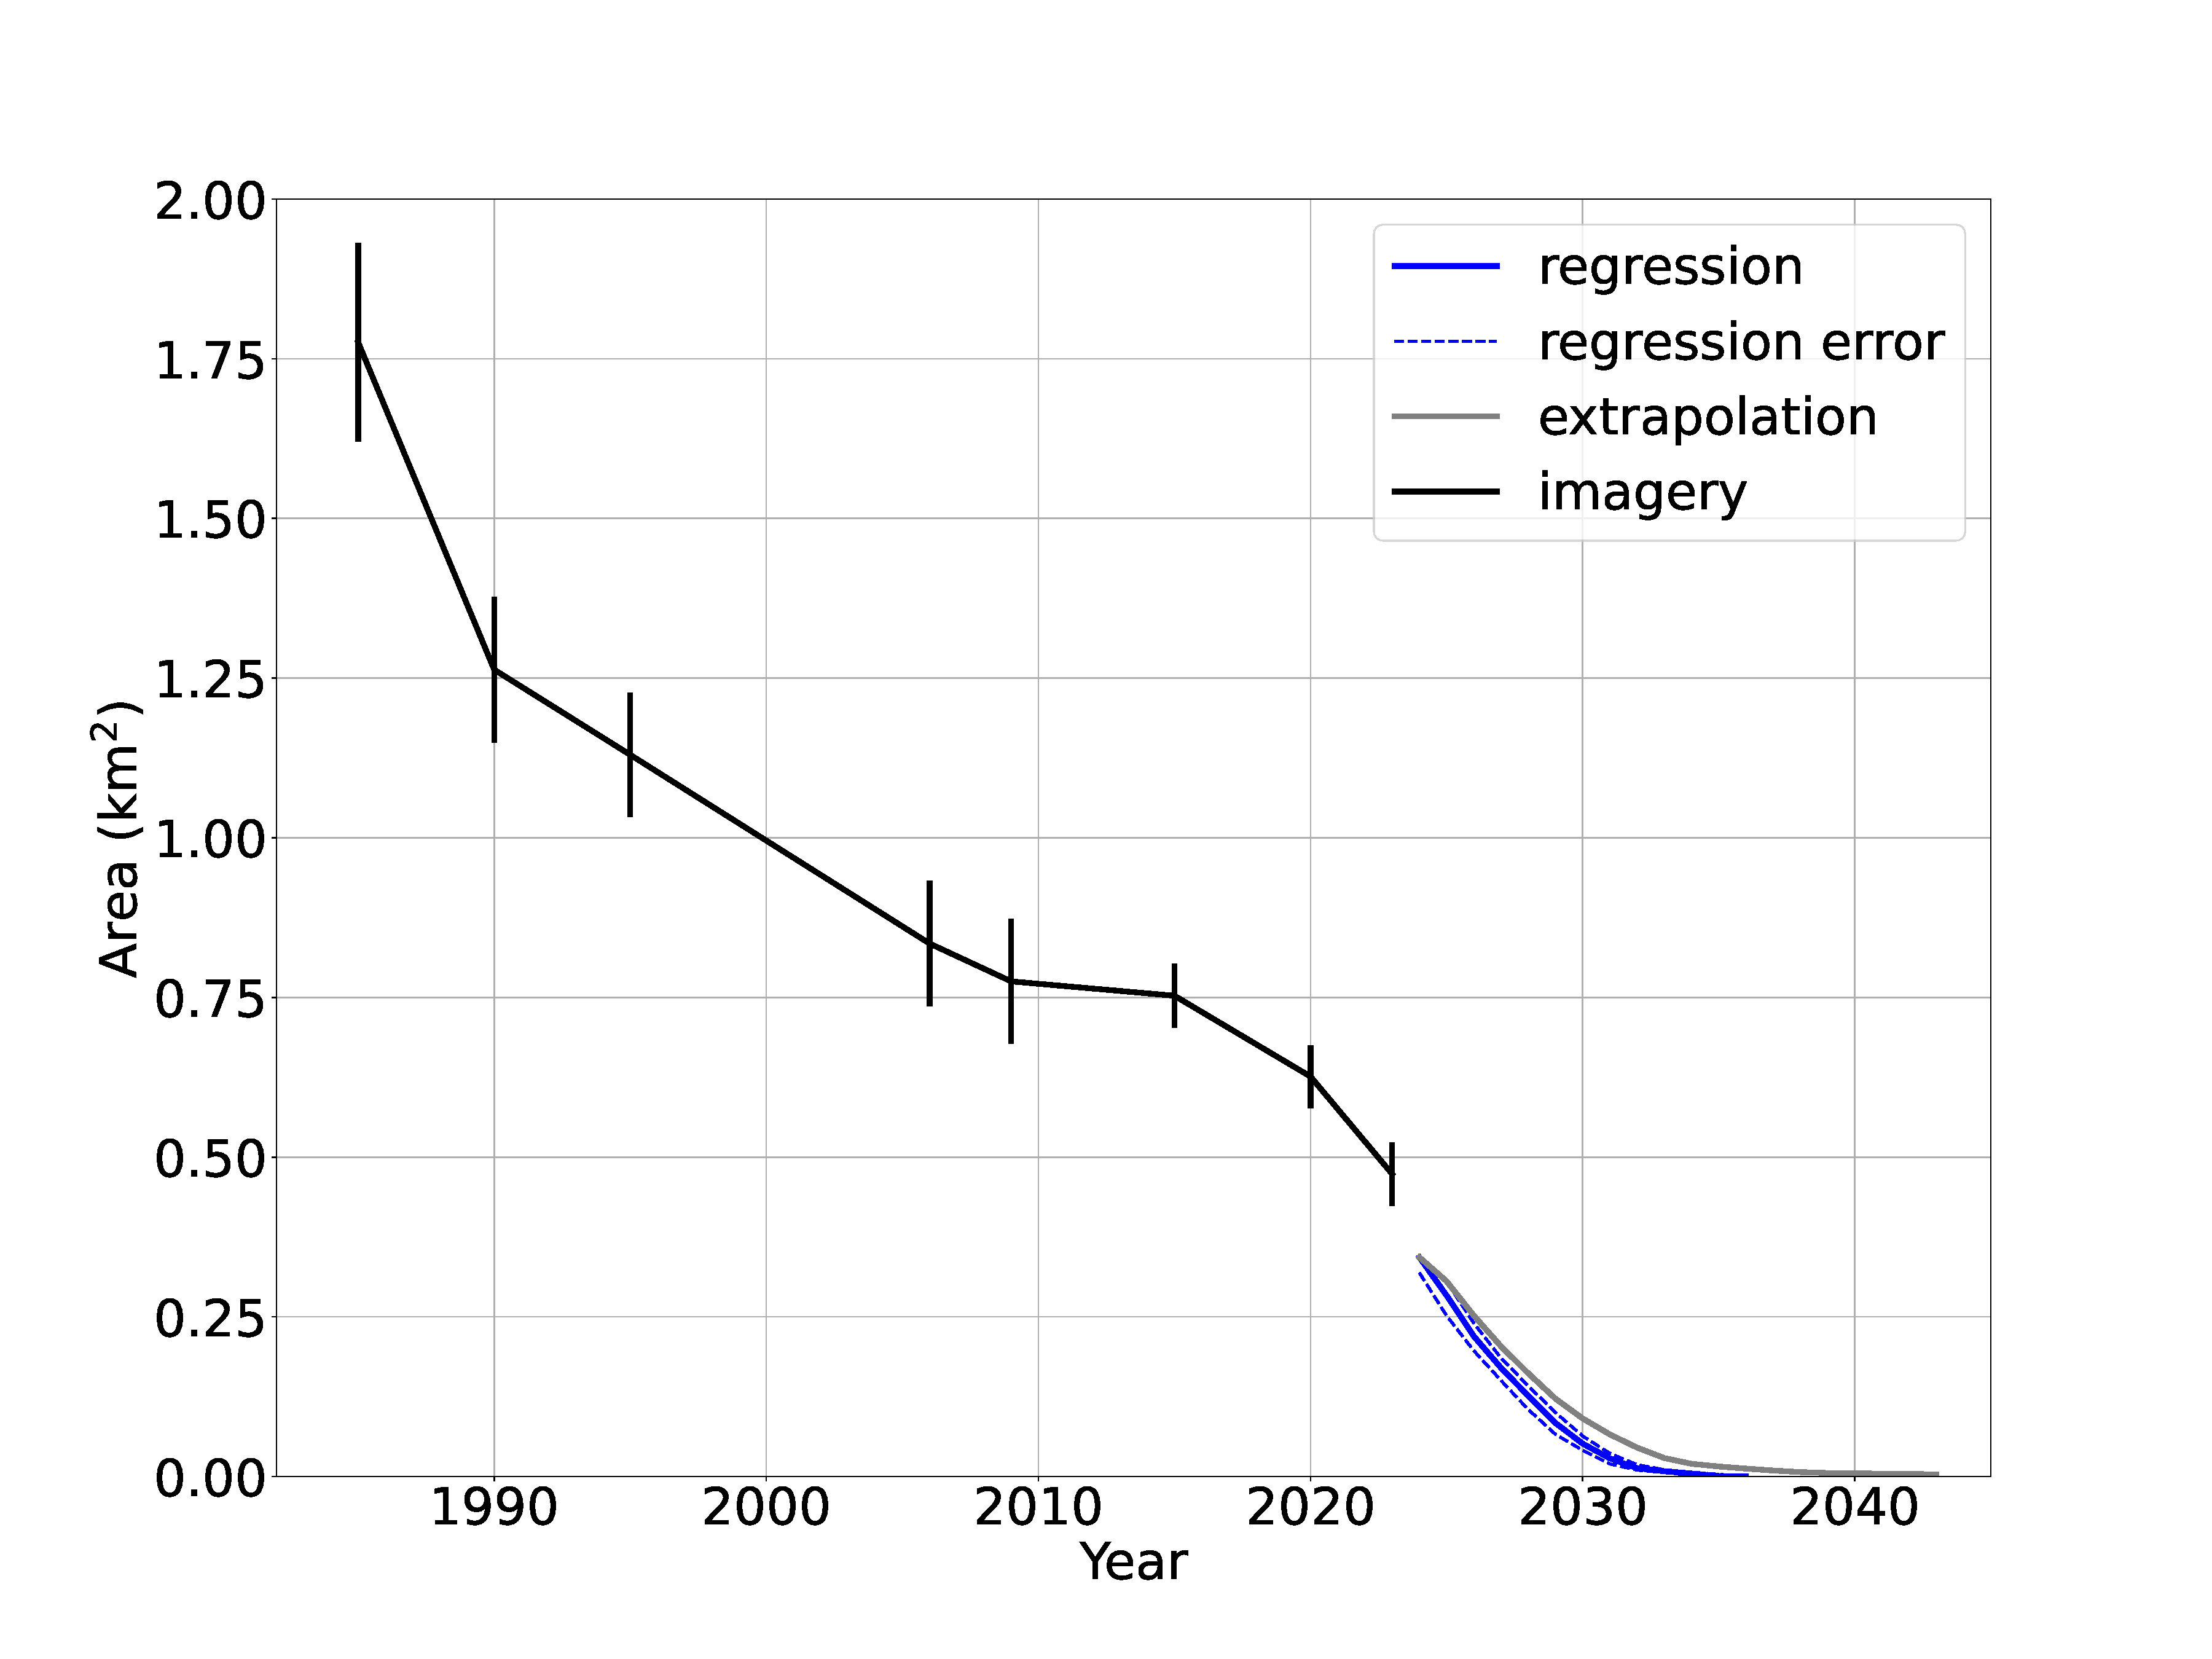
\includegraphics[width=86mm,trim=2.5cm 2cm 2.5cm 2cm, clip=true]
{area_through_time.pdf}
\caption{Modelled and observed glacier area change through time. Vertical bars are uncertainty in area as the product of the image resolution and glacier area. Results for the regression analysis (blue line) are bracketed by intializing the model with the error bounds on ice thickness. Error bounds for the elevation change extrapolation (gray line) are not shown, but are similar in spread to the regression uncertainty.}
\label{area}
\end{figure}

\begin{figure}[H]
\centering
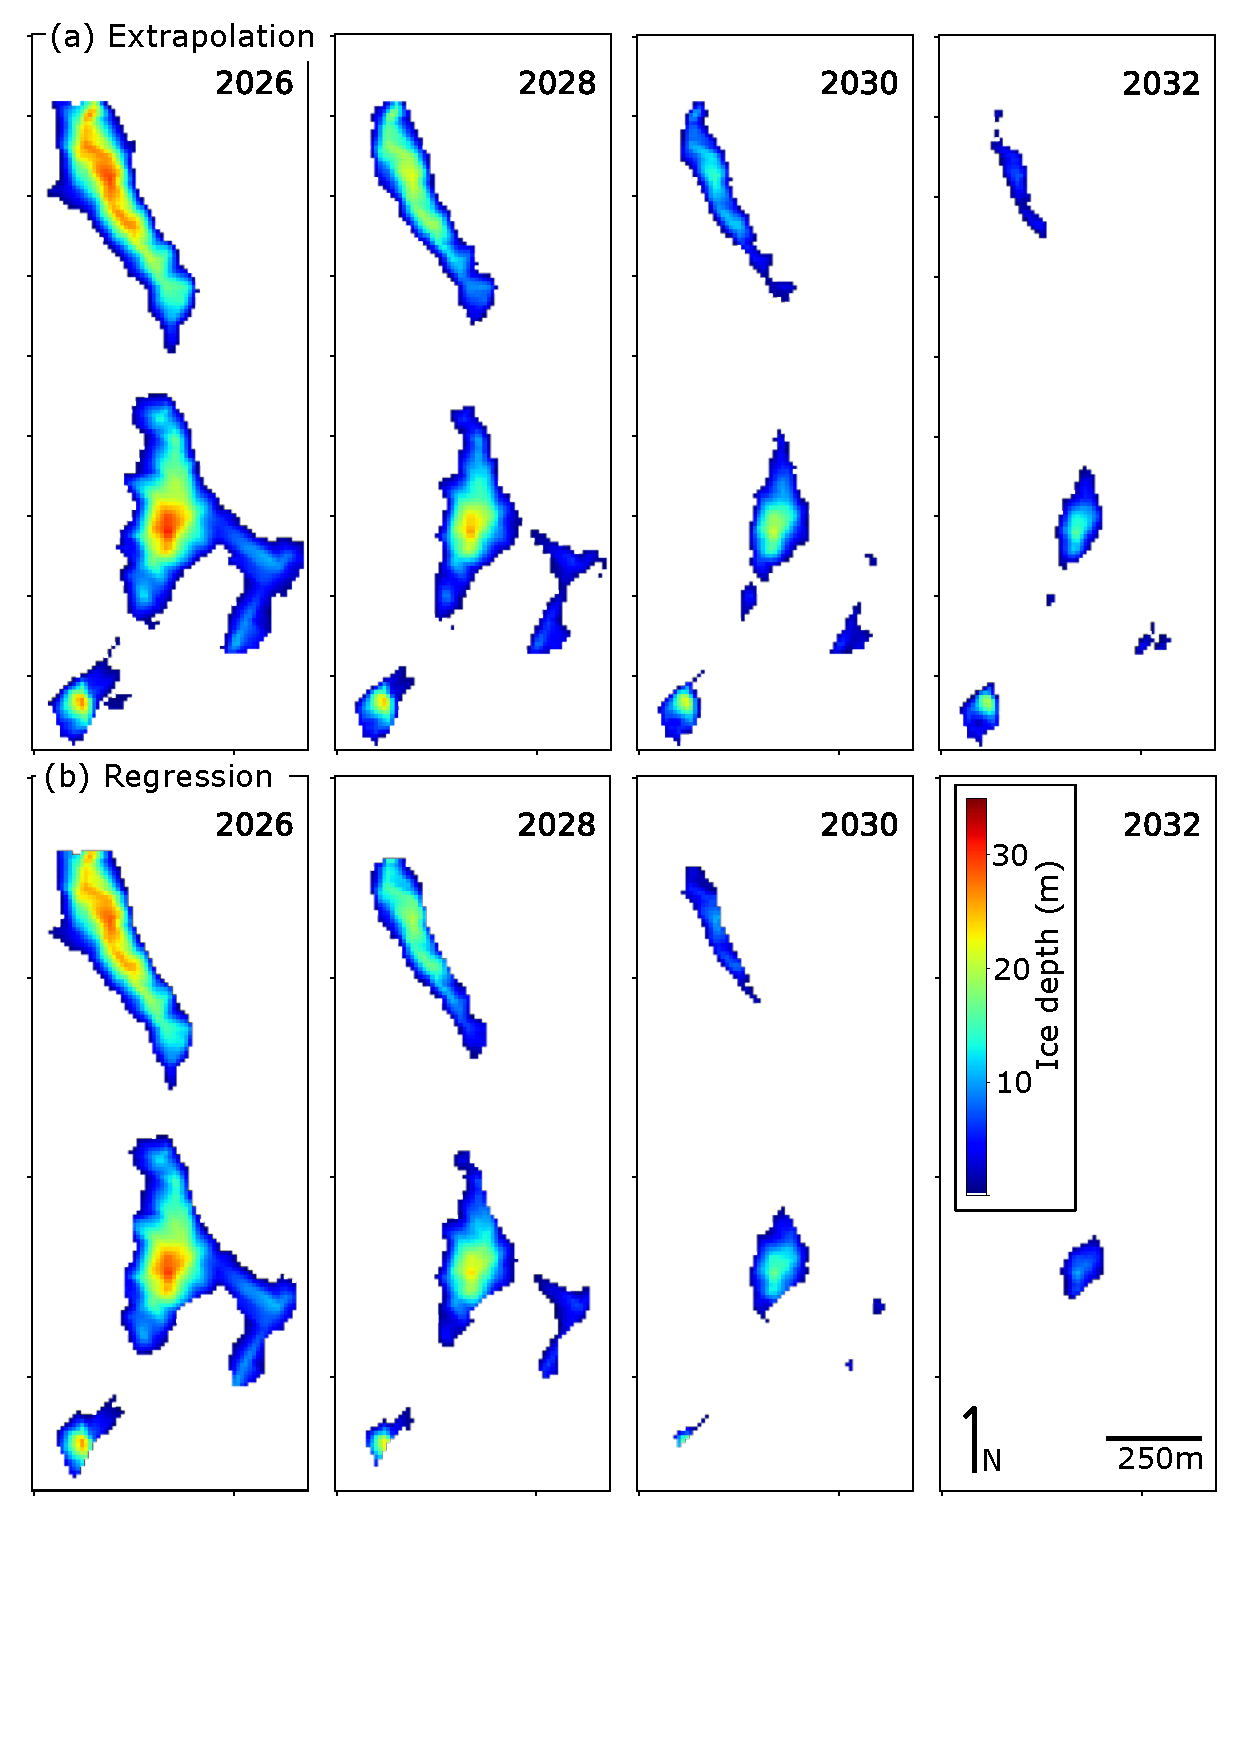
\includegraphics[width=86mm,trim=0cm 4.3cm 0cm 0cm, clip=true]
{forward.pdf}
\caption{Forward model of glacier area and thickness by (a - top panels) extrapolation of mean elevation change field between 2020 and 2024 and (b - bottom panels) multivariate regression.}
\label{loss_map}
\end{figure}

Calculating the specific balance from the 2024 reference surface shows that a net-zero balance can be achieved with an increase in precipitation of 1.5\,m\,w.e. (36\% mean winter snow accumulation) at the current temperature, or a change in temperature of -6.8$^\circ$C (95\% mean winter snow accumulation) at the current accumulation (Fig. \ref{SMB} a). By allowing the accumulation area to grow we compute a volumetric balance sensitivity that is slightly more optimistic (Fig. \ref{SMB} b), requiring an increase in precipitation of 1.1\,m\,w.e. (28\%) at the current temperature, or a change in temperature of -5.1$^\circ$C (71\%). 

For current conditions at Helm glacier, we compute a sensitivity to temperature as $\mathrm{C_T = -0.65 m\,w.e.\,yr^{-1}\,^\circ C^{-1}}$ while the sensitivity to accumulation is $\mathrm{C_P = 0.97 m\,w.e.\,yr^{-1}\,m\,w.e.^{-1}}$. On a unit-by-unit basis, the glacier is therefore 1.5 times more sensitive to changes in winter accumulation relative to changes in mean summer temperature. However, comparing the sensitivities by percentage change yield $\mathrm{C_P/C_T}=0.84$. The mass balance sensitivities for both the volumetric and specific mass balance methods yield very similar results. Our modelled value of $\mathrm{C_T = -0.65 m\,w.e.\,yr^{-1}\,^\circ C^{-1}}$ is in agreement to the observed mass balance temperature sensitivity of $\mathrm{C_T = -0.64 m\,w.e.\,yr^{-1}\,^\circ C^{-1}}$. 

%\begin{figure}[H]
%\centering
%\includegraphics[width=172mm,trim=2.5cm 2cm 2.5cm 2cm, clip=true]
%{C:/Users/jcrompto/Documents/writing/Helm/figures/MLR_all_2D.pdf}
%\caption{}
%\label{r2}
%\end{figure}

\section{Discussion}

Both methods for projecting surface elevation change lead to a demise of Helm Glacier within the next decade. Applying the average elevation change forward in time (method 1) is slightly more conservative than the regression model (method 2) because surface parameters like slope, orientation and elevation that are updated at each yearly time step in the regression model create a positive feedback in melt rate, which is not captured with the simple extrapolation. Like most glaciers, Helm glacier exhibits several intricacies that complicate a simple mass balance model or regression approach. For each melt season, modelled surface elevation change is generally underestimated along patches of the eastern margin where avalanche accumulation is exacerbated by valley wall shading. Elevation change is often overestimated at the eastern head of the glacier where snow redistribution by wind causes a reversal of the accumulation gradient. Linearly interpolating and extrapolating snow depth measurements to the snow depth field yields the best $R^2$ averaged across all observation periods, but in cases of extreme years for snow redistribution, a second or third-order polynomial fit can significantly increase the fit at high and low elevations for that year. Despite the uncertainties in ice thickness and nuances in melt, the glacier is thinning so rapidly that capturing subtleties in mass balance becomes increasingly irrelevant when trying to model the timing of extinction.

The linear regression model is driven by average temperatures over the past decade and an average snow accumulation field. As such, the forward model does not capture extreme melt events observed regionally and at Helm glacier. Examples of events and processes that likely make our projections conservative include the intense melt year of 2023 \citep{Menounos2025}, an equilibrium-line elevation that is starting to rise above the head of the glacier \citep{Bevington2025}, surface darkening from wildfire ash deposition that decreases ice albedo \citep{Menounos2025,AubryWake2022} and proglacial lake development leading to basal melt and calving \citep{Carrivick2013,Shugar2020}. These processes that we do not account for should lead to an overestimate of the temperature shift required to reach equilibrium mass balance (see Fig. \ref{SMB}). However, the temperature shifts that we derive in the sensitivity analyses are consistent with the observed increase in mean summer temperature of 4.6$^\circ$C from 1950 to present at the nearest ERA5-Land grid point. ERA5-Land reanalysis data does not show a statistically significant increase in precipitation that would otherwise contribute to the magnitude of disequilibrium for Helm glacier. 

%Given the maritime setting of Helm Glacier, it's sensitivity to changes in accumulation should be large relative to changes in temperature \citep{Letreguilly1988,Cuffey2010}. Although we can derive $\mathrm{C_T}$ and $\mathrm{C_P}$ from the model and $\mathrm{C_T}$ from observations, $\mathrm{C_P}$ cannot be derived from observation. However, from observations we derive a coefficient of determination between winter balance and specific net balance is only $R^2$=0.41, while the coefficient of determination between mean summer temperature and specific net balance is  $R^2$=0.6. A higher correlation between summer temperature and net balance than winter accumulation is consistent with alpine glaciers in Western Canada and USA, regardless of continentality \citep{Menounos2025}

\begin{figure}[H]
\centering
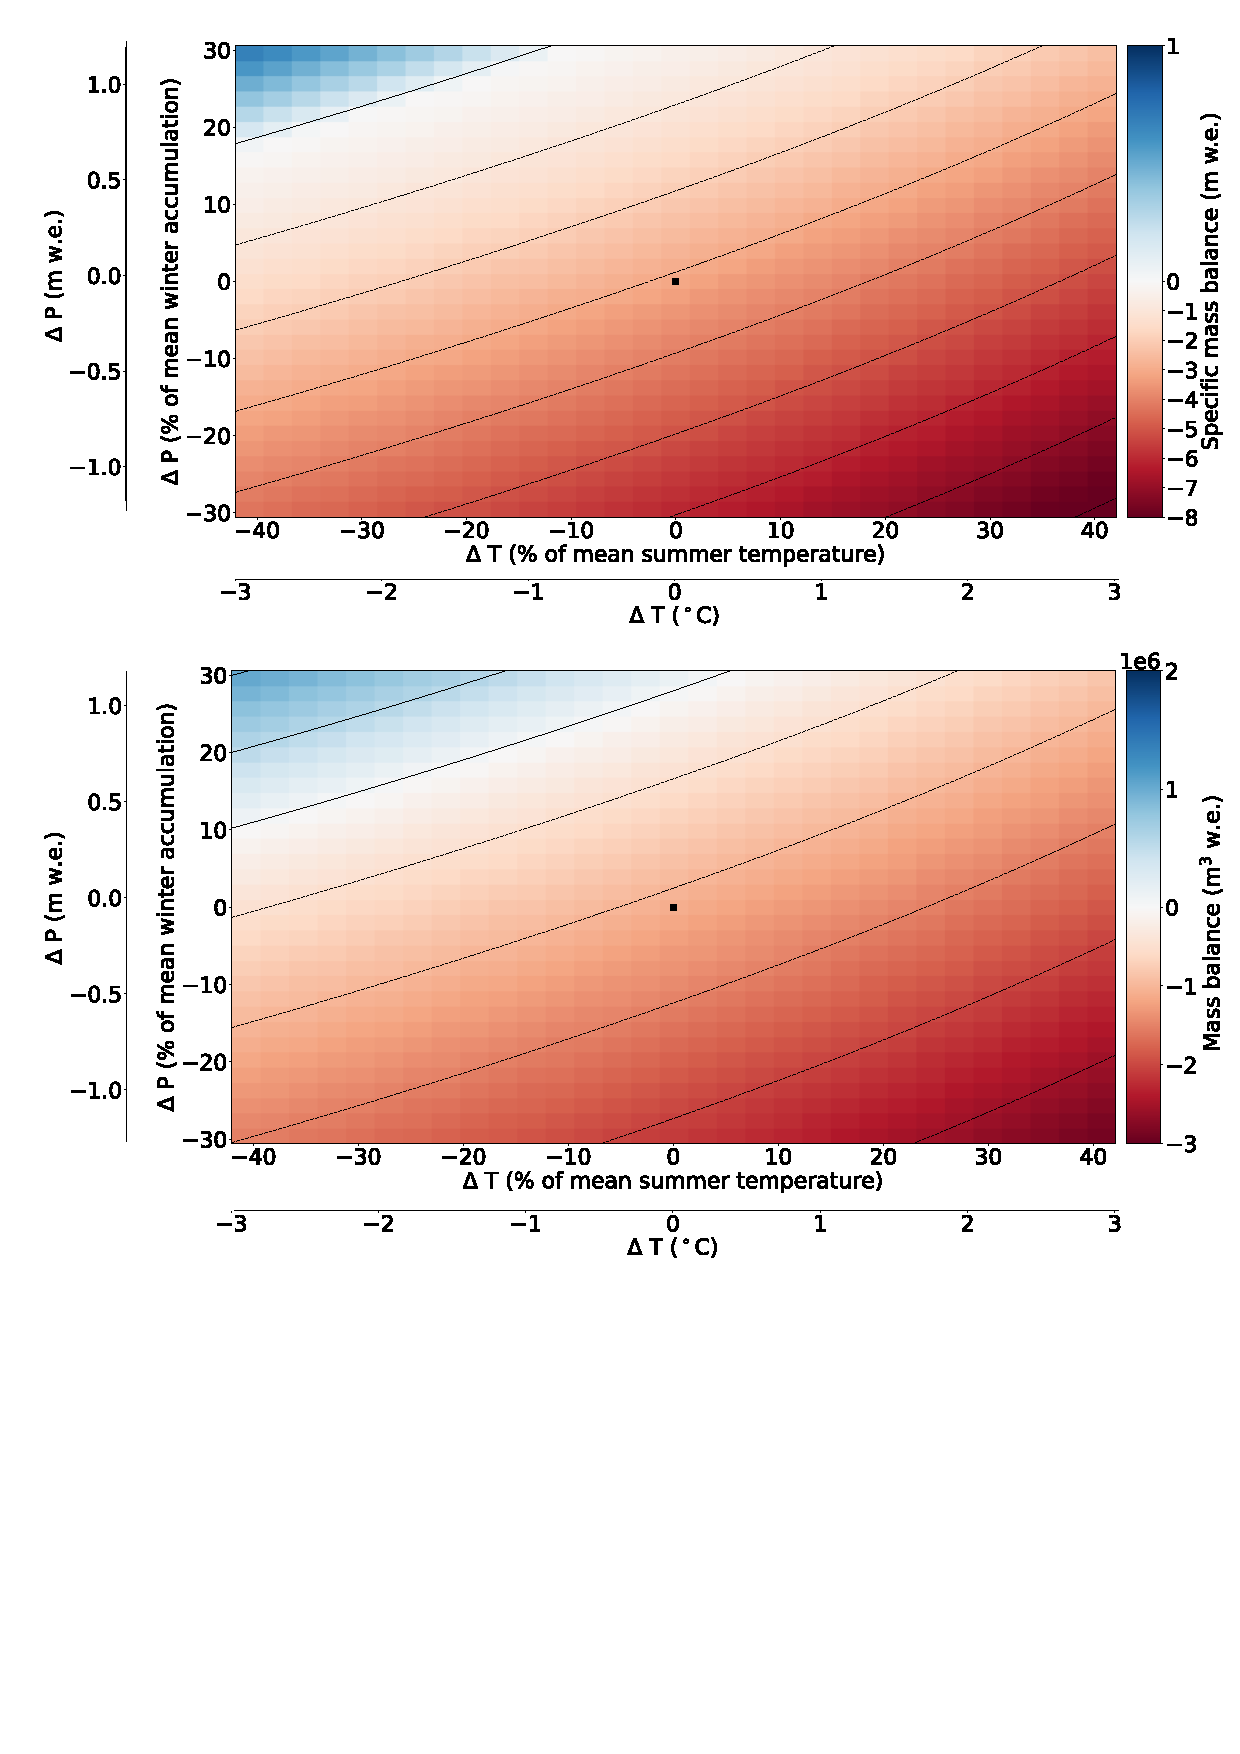
\includegraphics[width=86mm,trim=0cm 0cm 0cm 0cm, clip=true]
{SMB_S.pdf}
\caption{}
\label{SMB}
\end{figure}

\section{Conclusion}

\bibliography{refs}
\bibliographystyle{igs}


\end{document}
